% A simple Pentagon with TiKZ
% Author: Christoph Gerum <gerum@informatik.uni-tuebingen.de>

\documentclass{standalone}

\usepackage{tikz}


\begin{document}

%circle

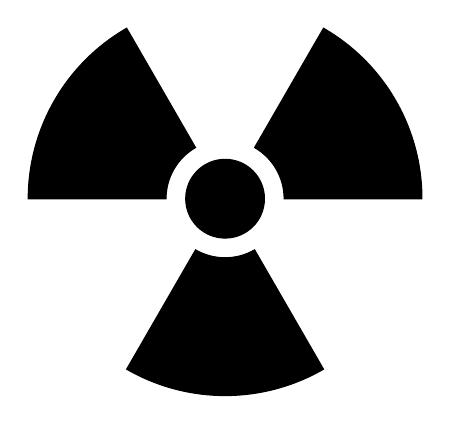
\begin{tikzpicture}[scale=0.5]
  \path (0,0) coordinate (origin);

  \draw [fill=black] (origin) circle (1cm);
  \draw [fill=black] (0:1.5 cm) -- (0:5cm) 
         arc(0:60:5cm) -- (60:1.5cm) arc(60:0:1.5cm) -- cycle;

  \draw [fill=black] (120:1.5 cm) -- (120:5cm)
         arc(120:180:5cm) -- (180:1.5cm) arc(180:120:1.5cm) -- cycle;
  
  \draw [fill=black] (240:1.5 cm) -- (240:5cm)
         arc(240:300:5cm) -- (300:1.5cm) arc(300:240:1.5cm) -- cycle ;
  
  
\end{tikzpicture} 

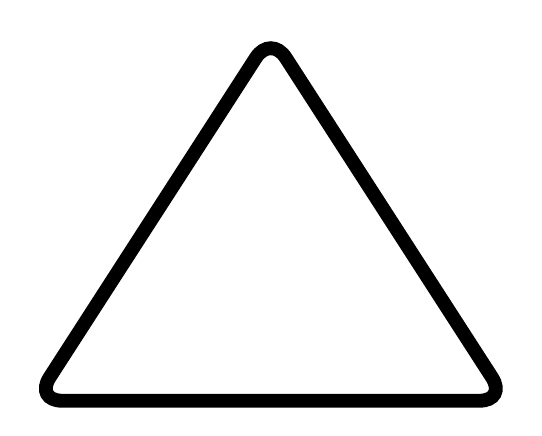
\begin{tikzpicture}[scale=0.3]
  \draw [line width=5pt, rounded corners=10pt] (-10,-5.5) -- (10,-5.5) -- (0, 10) -- cycle;
\end{tikzpicture}

\end{document}
